\documentclass{article}
\usepackage[margin=1.0in]{geometry}
\usepackage{titling}
\usepackage{graphicx}
\usepackage{float}
\usepackage[T1]{fontenc}
\begin{document}
	
	%%% title
	\setlength{\droptitle}{-5em}
	\title{1.6 Vertical Angles}
	\date{}
	\author{}
	\maketitle
	
	%%% first section
	\section{Definition}
	Each of the pairs of opposite angles made by two intersecting lines.  \newline They are congruent
	\section{Examples}
	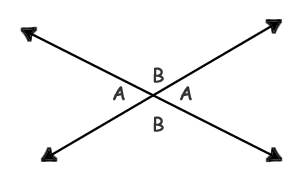
\includegraphics{pics/verticalangles.png}
	\newline A = A and B = B because of this
	
\end{document}